\documentclass{llncs}
%\usepackage{lncs}

\usepackage{amsmath,latexsym,amsfonts,amssymb,theorem}
\usepackage{rotating,graphs,stmaryrd}
\usepackage{subfig,pgf,xcolor,tikz}
\usepackage{cite}

% MISC ----------------------------------

\newcommand{\red}[1]{\textcolor{red}{#1}}
\newcommand{\blue}[1]{\textcolor{blue}{#1}}
\newcommand{\ttt}{\texttt}
\newcommand{\csp}{\hspace{.2em}}


% FORMULAS ------------------------------------

\newcommand{\mylabel}[1]{ \left\{
 \begin{array}{@{}l@{}} #1 \end{array} \right\}
}

\newcommand{\lvar}[1]{\mathtt{#1}}

\newcommand{\Z}{\mathbb{Z}}
\newcommand{\N}{\mathbb{N}}

\newcommand{\mtt}{\mathtt}
\newcommand{\mrm}{\mathrm}
\newcommand{\msf}{\mathsf}

\newcommand{\C}{\mathrm{Char}}
\newcommand{\Adr}{\mathrm{Adr}}
\newcommand{\Prog}{\mathrm{P}}

\newcommand{\fail}{\mathrm{fail}}
\newcommand{\g}{\mathrm{gra}}
\newcommand{\reg}{\mathrm{reg}}
\newcommand{\s}{\mathrm{s}}

\newcommand{\R}{\mathcal{R}}
\renewcommand{\L}{\mathcal{L}}
\newcommand{\I}{\mathcal{I}}
\newcommand{\G}{\mathcal{G}}
\newcommand{\A}{\mathcal{A}}
\renewcommand{\S}{\mathcal{S}}

\newcommand{\sos}{\mathrm{sos}}
\newcommand{\Sem}[1]{\llbracket{#1}\rrbracket}
\newcommand{\trans}[1]{\tau\llbracket{#1}\rrbracket}
\newcommand{\Gbot}{\mathcal{G}_{\bot}}

\newcommand{\X}{\mathrm{X}}
\newcommand{\V}{\mathrm{V}}
\newcommand{\E}{\mathrm{E}}
\newcommand{\D}{\mathrm{D}}
\newcommand{\tuple}[1]{\langle#1\rangle}
\newcommand{\la}{\langle}
\newcommand{\ra}{\rangle}
\newcommand{\dom}{\mathrm{Dom}}

\newcommand{\x}{\mathtt{x}}
\newcommand{\y}{\mathtt{y}}
\newcommand{\z}{\mathtt{z}}

\newcommand{\ifte}[3]{\mathtt{if}\ #1\ \mathtt{then}\ #2\ \mathtt{else}\ #3}
\newcommand{\ift}[2]{\mathtt{if}\ #1\ \mathtt{then}\ #2}
\newcommand{\tryt}[2]{\mathtt{try}\ #1\ \mathtt{then}\ #2}
\newcommand{\tryte}[3]{\mathtt{try}\ #1\ \mathtt{then}\ #2\ \mathtt{else}\ #3}
\newcommand{\noteq}{\mathrel{\text{\texttt{!=}}}}

\renewcommand{\bar}[1]{\overline{#1}}
\newcommand{\wt}[1]{\widetilde{#1}}
\newcommand{\wh}[1]{\widehat{#1}}

\newcommand{\ul}[1]{\underline{#1}}


% REWRITE RELATIONS ---------------------------

% Abstract reduction and term rewriting -------

\newcommand{\symto}{\leftrightarrow}

\newcommand{\DSto}{\mathop{\to}\limits}
\newcommand{\DSsymto}{\mathop{\symto}\limits}

\newcommand{\symredu}{\Leftrightarrow_{\R}}

\newcommand{\dder}{\Rightarrow}
\newcommand{\ldder}{\Leftarrow}
\newcommand{\der}{\Rightarrow^*}
\newcommand{\lder}{\Leftarrow^*}

\newcommand{\DSdder}{\mathop{\Rightarrow}\limits}
\newcommand{\DSldder}{\mathop{\Leftarrow}\limits}
\newcommand{\DSder}{\DSdder^*}
\newcommand{\DSlder}{\DSldder^*}

\newcommand{\DSlongdder}{\mathop{\Longrightarrow}\limits}
\newcommand{\DSllongdder}{\mathop{\Longleftarrow}\limits}


% GRAPHS -------------------------------------

\newcommand{\bluenodecolour}{\graphnodecolour(0,.6,1)}
\newcommand{\rednodecolour}{\graphnodecolour(1,.03,.03)}
\newcommand{\greennodecolour}{\graphnodecolour(0,1,0)}
\newcommand{\grey}{\graphnodecolour{.75}}
\newcommand{\dashed}{\graphlinedash{4 2}}

\newcommand{\script}{\scriptsize}
\newcommand{\fs}{\footnotesize}
\newcommand{\op}[3]{\textnode{#1}(#2){$\mathtt{#3}$}[\graphlinecolour{1}]}
\newcommand{\smallnode}{\graphnodesize{0.30}}
\newcommand{\nodegraph}[1]{% 
 \graphlinewidth{.01}
 \graphlinecolour{0}
 \graphnodecolour{1}
 \graphnodesize{.4}
 \begin{graph}(.4,.2)
  \roundnode{n}(.2,.1)\autonodetext{n}{#1}
 \end{graph}
}
\newcommand{\edgegraph}{% 
 \graphlinewidth{.01}
 \graphlinecolour{0}
 \graphnodecolour{1}
 \graphnodesize{.2}
 \grapharrowlength{.15}
 \grapharrowwidth{.45}
 \begin{graph}(1,.2)
  \roundnode{s}(.2,.1)\autonodetext{s}[s]{\tiny $s$}
  \roundnode{t}(.8,.1)\autonodetext{t}[s]{\tiny $t$}
  \diredge{s}{t}
 \end{graph}
}
\newcommand{\parrule}{% 
 \graphlinewidth{.01}
 \graphlinecolour{0}
 \graphnodecolour{1}
 \graphnodesize{.2}
 \grapharrowlength{.15}
 \grapharrowwidth{.45}
 \begin{graph}(.8,.2)
  \freetext(.6,0){par:}
 \end{graph}
 \begin{graph}(1,.2)
  \roundnode{s}(.2,.1)\autonodetext{s}[s]{\tiny 1}
  \roundnode{t}(.8,.1)\autonodetext{t}[s]{\tiny 2}
  \dirbow{s}{t}{.1}
  \dirbow{s}{t}{-.1}
 \end{graph}
 \begin{graph}(.4,.2)
  \freetext(.2,.1){\small $\dder$}
 \end{graph}
 \begin{graph}(1,.2)
  \roundnode{s}(.2,.1)\autonodetext{s}[s]{\tiny 1}
  \roundnode{t}(.8,.1)\autonodetext{t}[s]{\tiny 2}
  \diredge{s}{t}
 \end{graph}
}
\newcommand{\seqrule}{% 
 \graphlinewidth{.01}
 \graphlinecolour{0}
 \graphnodecolour{1}
 \graphnodesize{.2}
 \grapharrowlength{.15}
 \grapharrowwidth{.45}
 \begin{graph}(.8,.2)
  \freetext(.6,0){seq:}
 \end{graph}
 \begin{graph}(1.6,.2)
  \roundnode{s}(.2,.1)\autonodetext{s}[s]{\tiny 1}
  \roundnode{d}(.8,.1)
  \roundnode{t}(1.4,.1)\autonodetext{t}[s]{\tiny 2}
  \diredge{s}{d}
  \diredge{d}{t}
 \end{graph}
 \begin{graph}(.4,.2)
  \freetext(.2,.1){\small $\dder$}
 \end{graph}
 \begin{graph}(1,.2)
  \roundnode{s}(.2,.1)\autonodetext{s}[s]{\tiny 1}
  \roundnode{t}(.8,.1)\autonodetext{t}[s]{\tiny 2}
  \diredge{s}{t}
 \end{graph}
}


\usetikzlibrary{arrows,fit,backgrounds}
\tikzset{arrowin/.style={<-,>=latex,semithick},arrowout/.style={->,>=latex,semithick},root/.style={circle,draw,line width=2pt},box/.style={rectangle, minimum width=1cm, minimum height=1cm,text centered, draw=black}}


\begin{document}

\title{A Reference Interpreter for the Graph Programming Language GP2}
%\title{A Reference Interpreter for the Graph Programming Language}

\author{Christopher Bak, Glyn Faulkner, Detlef Plump and Colin Runciman} 
\institute{Department of Computer Science\\
           The University of York, UK}


\maketitle
\thispagestyle{empty}


\begin{abstract}
GP2 is an experimental programming language
for computing by graph transformation.
An initial interpreter for GP2, written
in the functional language Haskell, provides
a concise and simply structured reference
implementation.
Despite its simplicity, the performance of
the interpreter is sufficient for the
comparative investigation of a range of test
programs.
It also provides a platform for the development
of more sophisticated implementations.
\end{abstract}

\section{Introduction}

GP 2 is an experimental programming language in which the major part of
the computational state is a labelled directed graph, and the basic
units by which computational progress is made are subgraph-rewriting
rules.
Choices of rules and subgraphs are non-determinstic, and some of
the control structures above the level of rules involve back-tracking.

The implementation of such a programming language poses some
interesting challenges and opportunities.
Our ultimate goal is to produce a compiler from GP 2 to
high-performance executable code.
This paper reports a first stage towards that goal, the development
of a \emph{reference interpreter} for GP 2.
By this we mean an interpreter written with the main aim of
being clear, concise and correct.
Where there are design choices, simplicity of
definition takes priority over other considerations
such as performance and the richness of functionality.

Section~\ref{sec:gp2language} outlines and illustrates the GP 2 language
graph-programming language.
Section~\ref{sec:benchmark} presents a small set of test programs
written in GP 2.
Section~\ref{sec:usesrequirements} considers the uses and requirements
for a reference interpreter.
Section~\ref{sec:implementation} describes our reference interpreter for
GP 2.
Section~\ref{sec:results} sets out the results of using the reference
interpreter to evaluate the test programs in Section~\ref{sec:benchmark},
including various measures of the sizes of computations and the
resources needed for them.
Section~\ref{sec:conclusionsfuture} offers conclusions and indicates
likely lines of future work.


\section{Graph Programs}
\label{sec:graph-programs}

We give a brief introduction to GP, mainly by example (see \cite{Plump12a} for a language definition). A graph program consists of declarations of conditional graph transformation rules and macros, and exactly one main command sequence. Graphs are directed and may contain  loops and parallel edges. The rules operate on a \emph{host graph}\/ (or input graph) whose nodes and edges are labelled with lists consisting of integers and character strings.

Labels are of type \texttt{int} (for integers), \texttt{string} (for character strings), \texttt{atom} or \texttt{list}, where \texttt{atom} is the union of \texttt{int} and \texttt{string}. Atoms are considered as lists of length one, hence integers and strings are also lists. Given lists $\mtt{x}$ and $\mtt{y}$, their concatenation is written \texttt{x:y} (not to be confused with the append operation in Haskell). 
We proceed by discussing two example programs.

\begin{example}[Transitive Closure]
The principal programming construct in GP are conditional graph transformation rules labelled with expressions. The program in Figure \ref{fig:transitive-closure} applies the single rule \ttt{link} as long possible to a host graph. In general, any subprogram can be iterated with the \ttt{!}-loop.

\begin{figure}[htb]
\begin{center}
 \input{Programs/trans_closure.prog}
\end{center}
%\vspace{-.5\baselineskip}
\caption{Program for transitive closure}\label{fig:transitive-closure}
\end{figure}

Applying \ttt{link} amounts to non-deterministically selecting a subgraph of the host graph that matches \ttt{link}'s left graph, and adding to it an edge from node 1 to node 3 provided there exits no such edge (with any label). The application condition ensures that the program terminates and extends the host graph with a minimal number of edges.

It is not difficult to see that given any graph $G$, the program produces the smallest transitive graph that results from adding unlabelled edges to $G$.\footnote{``Unlabelled'' edges are actually labelled with the empty list.} Note that this graph is unique up to isomorphism and requires at most $n^2$ applications of \ttt{link}, where $n$\/ is the number of nodes in $G$. \qed
\end{example}
  

\begin{example}[Vertex Colouring]
The program in Figure \ref{fig:vertex-colouring} assigns a \emph{colour}\/ to each node of the host graph, such that non-loop edges have differently coloured endpoints. Positive integers are used as colours. The program replaces each node label $l$\/ with $l{:}i$, where $i$\/ is the node's colour. In addition, the rule \ttt{init} shades nodes to prevent being applied twice to a node. (Nodes can be graphically \emph{marked}\/ using shading or the colours red, green or blue.)

\begin{figure}[htb]
\begin{center}
 \input{Programs/vertex-colouring.prog}
\end{center}
%\vspace{-.5\baselineskip}
\caption{Program for vertex colouring}\label{fig:vertex-colouring}
\end{figure}

Rule \ttt{inc} is applied to the host graph as long as there are edges with identically coloured endpoints. It can can be shown that this terminates after at most $n^2$ rule applications, where $n$\/ is the number of nodes. In contrast to the previous example program, different graphs may result from this process. In particular, there is no guarantee that the number of colours produced is minimal. For instance, Figure \ref{fig:colour_results} shows two different colourings produced for the same host graph.
\qed
\end{example}

\begin{figure}[htb]
\begin{center}
 \input{Graphs/colour_results.graph}
\end{center}
%\vspace{-.5\baselineskip}
\caption{Different outputs from vertex colouring}\label{fig:colour_results}
\end{figure}

A GP command not used in the example programs is a rule set $\mtt{\{}r_1,\dots,r_n\mtt{\}}$. This command non-deterministically applies any of the rules to the current graph. The application \emph{fails}\/ if none of the left-hand graphs in the rules matches a subgraph. Matches must be injective and are only valid if they do not result in dangling edges.

Another construct not yet discussed is the branching command \ttt{if} $C$ \ttt{then} $P$ \ttt{else} $Q$, where $C$, $P$ and $Q$ are arbitrary command sequences. This is executed on a host graph $G$ by first executing $C$ on a copy of $G$. If this results in a graph, $P$\/ is executed on the original graph $G$; otherwise, if $C$ fails, $Q$ is executed on $G$. The command \ttt{try} $C$ \ttt{then} $P$ \ttt{else} $Q$ has a similar effect, except that $P$\/ is executed on the graph resulting from $C$'s execution. 

\section{Benchmark Programs}
\label{sec:benchmark}
 
We envisage GP 2 as a general-purpose language for graph problems, hence the reference interpreter should be tested on algorithms of varying complexity. This is different from the benchmarking reported in \cite{Varro-Schuerr-Varro05a} which focusses on a deterministic program with very limited complexity. In Section \ref{sec:performanceevaluation}, we evaluate the performance of our interpreter on a small set of benchmark programs. These include the programs for transitive closure and vertex colouring, and three more programs which we describe in this section.

\vspace{.5\baselineskip}
\noindent
\emph{Shortest distances.} The program in Figure \ref{fig:shortest-distances} expects an input graph $G$\/ containing a unique grey node $s$, where edge labels are assumed to be non-negative integers. A unique output graph is obtained by marking grey each node reachable from $s$ and replacing its label $l$\/ with $l{:}d$, where $d$\/ is the shortest distance from $s$. (A distance is the sum of the edge labels of a directed path.)
  
The program first assigns distance 0 to the unique start node $s$. Then the loop \ttt{add!} traverses the nodes reachable from $s$, assigning distances by adding edge labels. In a second phase, the loop \ttt{reduce!} minimizes distances by searching for edges whose sum of source node distance and edge label is smaller than the target node distance, and replacing the target node distance with the sum.

\begin{figure}[t]
\begin{center}
\input{Programs/distances.prog}
\end{center}
\caption{Program for shortest distances}\label{fig:shortest-distances}
\end{figure}

The requirement that edge labels are non-negative ensures that the program terminates. It can be relaxed by allowing negative edge labels but requiring that directed cycles have a non-negative overall distance.

\begin{figure}[t]
\begin{center}
\input{Programs/acyclic.prog}
\end{center}
\caption{Program for recognising acyclic graphs}\label{fig:acyclicity}
\end{figure}
\vspace{.5\baselineskip}
\noindent
\emph{Recognising acyclic graphs.} The program in Figure \ref{fig:acyclicity} checks whether its input graph is acyclic. If this is the case, the program preserves its input graph, otherwise it fails. Suppose we call the program \ttt{acyclic} to use it as a macro in the program \ttt{if} \ttt{acyclic} \ttt{then} $P$ \ttt{else} $Q$. Given any input graph $G$, this program will test whether $G$\/ is acyclic and, depending on the result, either execute $P$ or $Q$ on $G$.  
  
The presence of cycles is checked by deleting as long as possible edges whose sources have no incoming edges, and testing whether any edges remain. This is correct since an application of \ttt{delete} preserves both the absence and the presence of cycles (by the condition of the rule). Moreover, a graph to which \ttt{delete} is not applicable is acyclic if and only if it is edge-less (every acyclic graph with edges must contain an edge to which \texttt{delete} is applicable). 

% \subsection{Rooted 2-colouring}
% 
% \begin{tabular}{lp{10.5cm}}
% \ul{Input:} & A connected graph $G$. \\
% \ul{Output:} & If $G$\/ is 2-colourable, then the output is obtained from $G$\% / by marking each node with either red or blue. The source and target of each % non-loop edge have different colours.\\
% & If $G$\/ is not 2-colourable, then the output is $G$.
% \end{tabular}
% 
% \vspace{10pt}
% 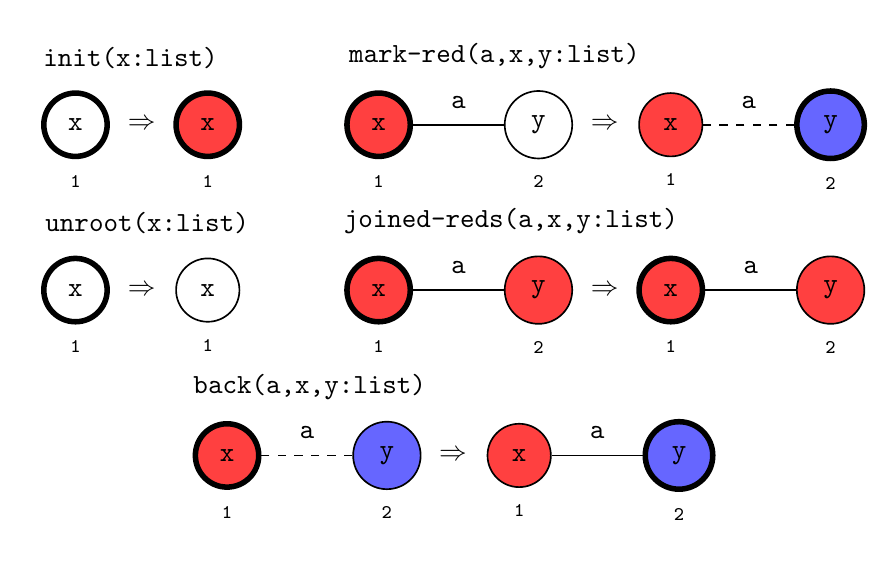
\begin{tikzpicture} [scale=0.7,align=center,auto,inner sep=2mm,arrowin,arrowout,font=\ttfamily]
%init
\node at (0,0)[root,label=below:\scriptsize{1}]{x};
\node at (1.2,0){$\Rightarrow$};
\node at (1,0)[above=5mm] {init(x:list)};
\node at (2.4,0)[root,fill=red!75,label=below:\scriptsize{1}]{x};

%unroot
\begin{scope}[yshift=-3cm]
\node (l1) at (0,0)[root,label=below:\scriptsize{1}]{x};
\node at (1.2,0){$\Rightarrow$};
\node at (1.3,0)[above=5mm] {unroot(x:list)};
\node (r1) at (2.4,0)[inner sep = 2mm,circle,draw,label=below:\scriptsize{1}]{x};
\end{scope}


%mark-red
\begin{scope}[xshift=5.5cm]
\node (l1) at (0,0)[root,fill=red!75,label=below:\scriptsize{1}]{x};
\node (l2) at (2.9,0)[inner sep = 2mm,circle,draw,label=below:\scriptsize{2}]{y}
   edge [-] node[above]{a} (l1);
\node at (4.1,0){$\Rightarrow$};
\node at (2.1,0)[above=5mm] {mark-red(a,x,y:list)};
\node (r1) at (5.3,0)[circle,draw,fill=red!75,label=below:\scriptsize{1}]{x};
\node (r2) at (8.2,0)[root,fill=blue!60,label=below:\scriptsize{2}]{y}
  edge [-,dashed] node[above]{a} (r1);  
\end{scope}

%joined-reds
\begin{scope}[xshift=5.5cm,yshift=-3cm]
\node (l1) at (0,0)[root,fill=red!75,label=below:\scriptsize{1}]{x};
\node (l2) at (2.9,0)[circle,draw,fill=red!75,label=below:\scriptsize{2}]{y}
  edge [-] node[above]{a} (l1);
\node at (4.1,0){$\Rightarrow$};
\node at (2.4,0)[above=5mm] {joined-reds(a,x,y:list)};
\node (r1) at (5.3,0)[root,fill=red!75,label=below:\scriptsize{1}]{x};
\node (r2) at (8.2,0)[circle,draw,fill=red!75,label=below:\scriptsize{2}]{y}
  edge [-] node[above]{a} (r1);
\end{scope}

%back
\begin{scope}[xshift=2.75cm,yshift=-6cm]
\node (l1) at (0,0)[root,fill=red!75,label=below:\scriptsize{1}]{x};
\node (l2) at (2.9,0)[circle,draw,fill=blue!60,label=below:\scriptsize{2}]{y}
  edge [-,dashed] node[above]{a} (l1);  
\node at (4.1,0){$\Rightarrow$};
\node at (1.5,0)[above=5mm] {back(a,x,y:list)};
\node (r1) at (5.3,0)[circle,draw,fill=red!75,label=below:\scriptsize{1}]{x};
\node (r2) at (8.2,0)[root,fill=blue!60,label=below:\scriptsize{2}]{y}
  edge [-] node[above]{a} (r1);
\end{scope}

\end{tikzpicture}
 \\
% \vspace{10pt}
% 
% \ul{Notes}
% \begin{enumerate}
% \setlength{\itemsep}{-.5ex}
% \item The nodes in rule \ttt{unroot} are violet. They can match a node of any % colour. A violet right-hand node takes the colour of the match of the left-han% d node.
% \item The edges in the \ttt{mark}, \ttt{joined} and \ttt{back} rules are \emph% {bidirectional}. They match host graph edges in either direction.
% \end{enumerate}


\vspace{.5\baselineskip}
\noindent
\emph{Generating Sierpinski triangles.} A \emph{Sierpinski triangle} is a self-similar geometric structure which can be recursively defined. Figure \ref{fig:sierpinski} shows a Sierpinski triangle of generation three, composed of three second-generation triangles, each of which consists of three triangles of generation one.\footnote{The geometric layout was created by the graphical interface of the GP 1 implementation \cite{Manning-Plump08b}.}

The program in Figure \ref{fig:Sierpinski-program} expects as input a single node labelled with the generation number of the Sierpinski triangle to be produced. The rule \texttt{init} creates the Sierpinski triangle of generation 0 and turns the input node into a ``control node'' with label $x{:}0$, holding the required generation number $x$ together with the current generation number.

\begin{figure}[p]
\begin{center}
\input{Programs/sierpinski.prog}
\end{center}
\caption{Program for generating Sierpinski triangles}\label{fig:Sierpinski-program}
 \begin{center}
  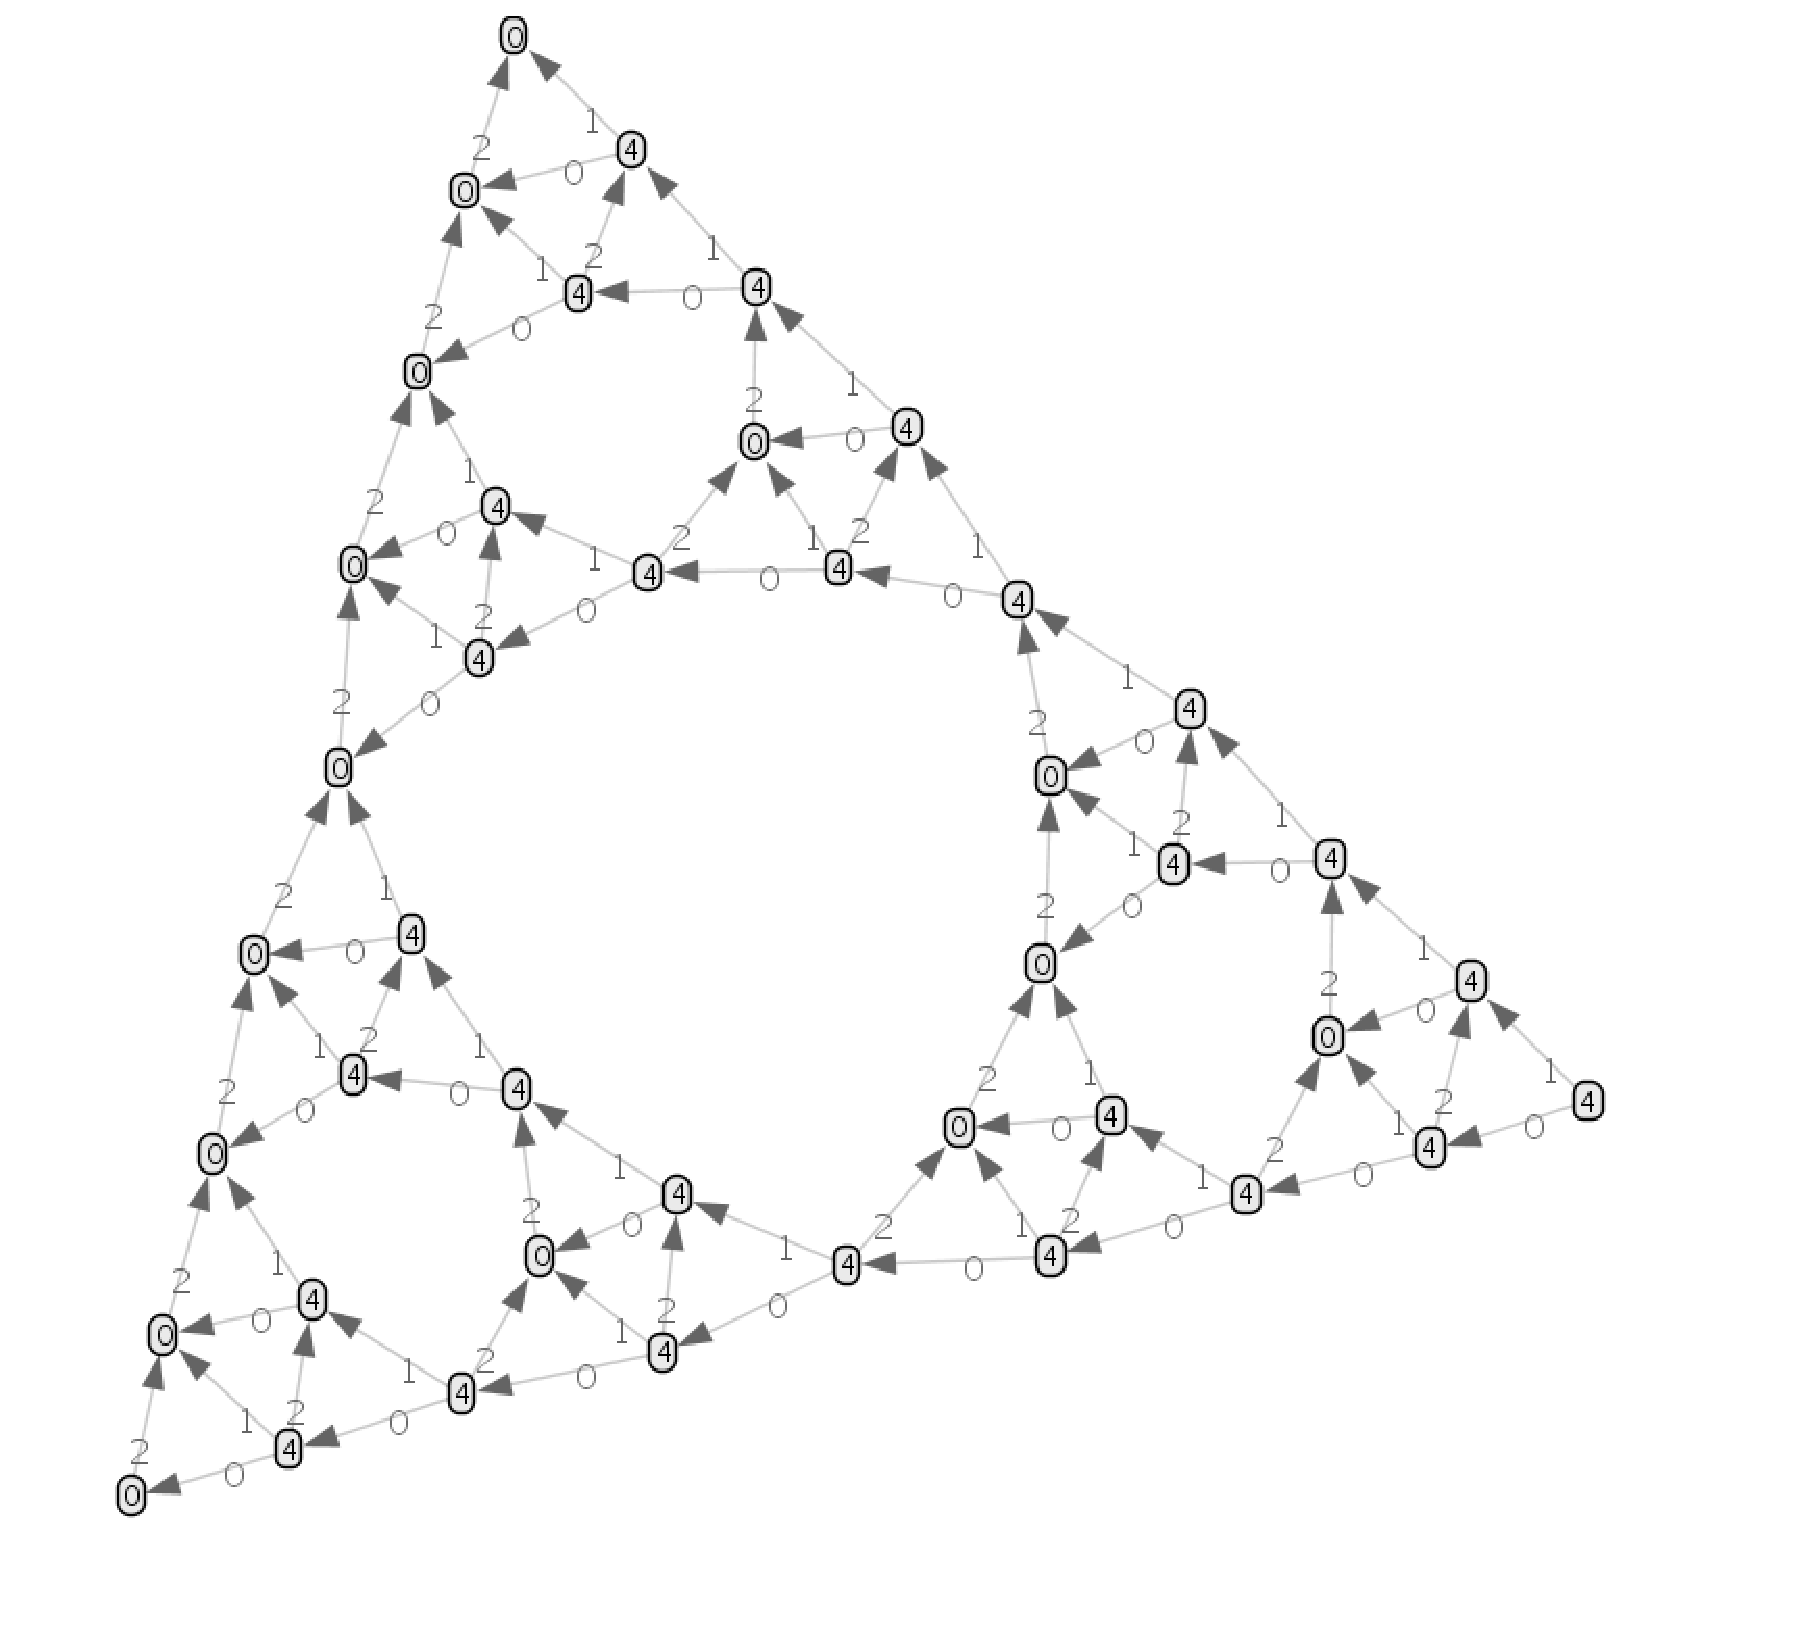
\includegraphics[scale=.35,angle=-15]{sierpinski-3.eps}
 \end{center}
\vspace*{-2.5cm}
\caption{Third generation Sierpinski triangle \label{fig:sierpinski}}
\end{figure}

After initialisation, the nested loop $\mtt{(inc;\, expand!)!}$ is executed. In each iteration of the outer loop, \texttt{inc} increases the current generation number if it is smaller than the required number (which is checked by the rule's condition). If the test is successful, the inner loop \ttt{expand!} performs a Sierpinski step on each triangle whose top node is labelled with the current generation number: the triangle is replaced by four triangles such that the top nodes of the three outer triangles are labelled with the next higher generation number. The test $\mathtt{x > y}$ fails when the required generation number has been reached. In this case the application of \texttt{inc} fails, causing the outer loop to terminate and return the current graph which is the Sierpinski triangle of the requested generation.

Sierpinski triangles pose a hard challenge for graph transformation: generating the $n$-th triangle requires space and a number of rule applications exponential in $n$. This problem was part of the 2007 tool contest for graph transformation, where the goal was to generate triangles of generation numbers as high as possible and as fast as possible \cite{Taentzer_et_al08a}.

\section{Reference Interpreters: Uses and Requirements}
\label{sec:usesrequirements}

A reference interpreter has several potential uses.
Each has consequences for the
way the reference interpreter is written and the
facilities it provides.

\paragraph{An arbiter for programmers}
A programmer working in a new language needs to
know whether what they are writing is a valid
program, and whether the effect of executing it
is the effect they intend.
To resolve such issues, the programmer may want to
use a reference interpreter as a black box,
checking the output it produces given their
program as input.
Or they may wish to consult some part of the
source-code for the interpreter, to know the exact
rule defining some aspect of the language they
are unsure about.

It follows that a reference interpreter should
provide as output at least a report whether a
program is valid, and if so a clear representation
of the result when it is evaluated.
It also follows that the source-code for a
reference interpreter should
be organised in such a way that salient components
are easy to identify.
For ease of reading it should be written using a
consistent style in a modest subset of a suitable
high-level language.

\paragraph{An arbiter for implementors}
An implementer of a programming language,
developing their own interpreter or compiler,
needs a standard against which to test the correctness
of their implementation.
There are two main respects in which any
implementation should agree with a reference interpreter
as a defining standard.
They should agree which programs are valid,
and for valid programs they should agree the results
of executing them.
Like application programmers, implementers too may
wish sometimes to use the reference interpreter as
a black box, but at other times to consult its
internal definitions. 

There are additional requirements for this use,
bearing in mind the likely development or generation
of many test programs.
The representation of the
reference interpreter's results for such programs
should be amenable to automated comparison.
This comparison presents particular challenges when
behaviour of programs may be non-deterministic,
or programs may not terminate, or both.
The number of test programs may be large
--- there may even be arbitrarily many test programs generated dynamically.
So although performance is not a design goal for the reference
interpreter, its performance should be good enough to
make such multi-test comparisons feasible.

\paragraph{A prototype for application developers}
If no production compiler has been developed for the language,
or none is yet available to an application developer,
they may need to use a reference interpreter as
an initial development platform.

During the development of application programs, errors
are common.
So, for this use, a reference interpreter should provide
not only a check for valid programs, but a rapid check
with informative reports of errors.
Yet elaborate error handling must not obscure the
definitional style in which the interpreter is written.
Similarly, it is desirable to have the option of some
kind of trace or other informative report to shed
light on failures or unexpected results when a program
is evaluated.
Here again, the machinery must not obsure the basic
definitions for evaluation, nor should it impose heavy
performance costs when performance of the interpreter
has already been sacrificed in favour of simplicity.

\paragraph{A prototype for implementation developers}
As well as using a reference interpreter to verify correctness,
implementers may wish to use it as the starting point in the
development of another interpreter or a compiler.
The whole course of such a development might even be defined as
the successive replacement of interpreter components by
alternatives giving higher performance, or richer information,
at the cost of greater complexity.
The advantage of this approach is that as each replacement
is introduced it can be checked as a new component in an already
tried system.

This use of a reference interpreter requires a
modular design with simple and clearly defined interfaces
between components.
Concerns should be separated so far as possible, avoiding
dependencies that are not strictly necessary.
Options for development by successive replacement may be further
increased by choosing a host programming system for the reference
interpreter that has a well-developed foreign-language interface. 



\section{The implementation}


\subsection{Data structures}

The reference interpreter uses a trivial implementation of an extensible array library, written initially without concern for performance issues, but encapsulated in such a way as to be replaceable with a more efficient library later if required. Specifically, a graph is represented as a pair of extensible arrays: one for the nodes and one for the edges.

\subsection{Program environment}

\subsection{Graph matching}

The graph matcher constructs a list of GraphMorphisms, where a GraphMorphism is a data structure containing the program environment, namely the variable-value assignments; a mapping between the NodeIds in the LHS of the rule graph and the corresponding NodeIds in the host graph; and a similar list of EdgeId mappings. Morphisms are generated by first constructing the set of all possible NodeMorphisms, then augmenting each node morphism with appropriate edge mappings. A NodeMorphism is a GraphMorphism without a list of EdgeId mappings.


The node matching algorithm takes as input the LHS L and the host graph G. It works as follows:

\begin{enumerate}
	\item Count the number of nodes k in L.
	\item Generate all sets of size k containing nodes from G.
	\item Iterate through the sets from step 2, comparing node labels in L to labels in G. Keep the sets in which node labels correspond for all pairs of nodes.
\end{enumerate}

It is clear that the complexity of this algorithm increases rapidly with both the size of L and the size of G. This is a naive matching strategy that would not be appropriate if performance were a consideration. In this case, where correctness is a greater concern, the simplicity of this algorithm is of benefit by making the source code easier to reason about.


The edge-matching algorithm takes as input the LHS L, the host graph G and a node morphisms NM. It works as follows:


\begin{enumerate}
	\item Get the source and target of each edge in L.
	\item Using NM, translate each source and target pair to the corresponding pair of host graph nodes.
	\item For each pair of host graph nodes (source, target), get the set of edges in G from source to target.
	\item Associate each edge in L with its set of candidate edge matches found in step 3.
	\item For all edges in L, test their label against the labels of each of its candidate matches. If the host label matches the LHS label (possibly with a variable-value assignment), add the assignment to the environment and add the edge match to the morphism. Otherwise, do nothing.
\end{enumerate}


Since it only generates edge sets that conform to the structural requirements of a graph morphism, it is more sophisticated than the node matching algorithm. The edge-matching algorithm has a smooth implementation due to features of Haskell. The first four steps are achieved with maps, ensuring that each LHS-edge is paired up with the correct set of host-edges.


\subsection{The dangling condition}

In the double-pushout framework of graph transformation, on which GP 2 is based, a rule may not be applicable for a particular match as applying the rule could leave an edge without a source or target. The dangling condition forbids this: it requires that all host edges not deleted by the rule are not incident to nodes deleted by the role.


\subsection{Isomorphism checking}

Producing all possible output graphs leads to the issue that many of the results may be isomorphic. To simplify analysis of the results, we implemented a basic isomorphism checker, so that our program completes with a set of all possible distinct output graphs, plus a count of the number of isomorphic variants of each graph that were seen.


\subsection{Rooted graphs}

Lessons learned from the implementation of the original GP language led to the addition of support for root nodes to GP2. A node carries a simple binary flag indicating whether it is a root node or not. A root node in a rule graph can only match a root node in the host graph, and then only if all other normal matching conditions are met, eliminating a large number of possible subgraph matches with only an inexpensive boolean test. Whereas a non-root node in the rule graph may match a node irrespective of its root-node status.


Even in the reference interpreter, addition of a root node can result in a significant performance gain of TODO.


\section{Performance Evaluation}
\label{sec:performanceevaluation}

In this section we will look at how efficiently our interpreter executes the benchmark programs described in Section \ref{sec:benchmark}, and discuss the factors that affect its performance. Though not tuned for speed, the interpreter must run fast enough to allow its use as a practical tool.


% TODO: mention performance of previous versions, and how increased performance brought bugs and limitations to light.


\subsection{The Test Environment}

We compiled the interpreter using The Glasgow Haskell Compiler\cite{ghc} version 7.6.3 with optimisations and profiling support enabled:

\begin{verbatim}
$ ghc -O2 -prof -fprof-auto -rtsopts -o gp2 Main.hs
\end{verbatim}

All figures reported were obtained using a quad-core Intel i7 clocked at 3.4GHz, with 8GB RAM, running 64-bit Ubuntu 14.04 LTS with kernel 3.13.0. The number of processor cores should not have a significant effect on the measured performance of the single-threaded GP~2 interpreter.

We ran benchmarks using the following command

\begin{verbatim}
$ timeout --foreground 5m time \
      gp2 +RTS -p -sgc.prof -RTS $GPOPT $PROG $GRAPH 10000
\end{verbatim}

\noindent
limiting execution time to five minutes for each application of a program to a host graph. We used the sum of user and system time reported by the standard \texttt{time} utility as our measure of execution time.
The arguments to \texttt{gp2} between \texttt{+RTS} and \texttt{-RTS} tell the Haskell run-time system to save profiling information.  The \texttt{\$GPOPT} variable was either set to \texttt{--one} to put the interpreter into single-result mode (see Table \ref{table:resultsSingle}), or unset for all-result mode (see Table \ref{table:resultsAll}).
The final three mandatory arguments to the \texttt{gp2} executable specify the benchmark program, the host graph, and the maximum number of rule applications, as described in Section \ref{sec:implementation}.

\subsection{Host Graphs}
\label{subsec:hosts}

The names of host graphs used for benchmarking give an indication of their structure.

\vspace{.5\baselineskip}
\noindent
\emph{Gen $n$}. The \textit{Sierpinski} program expects a host graph containing a single node with a numeric label, which controls the number of iterations of the \texttt{expand!} command.

\vspace{.5\baselineskip}
\noindent
\emph{Linear $n$}. A chain of $n$ nodes. The first node has only a single outgoing edge. The last node has only a single incoming edge. All other nodes have exactly one incoming and one outgoing edge.

\vspace{.5\baselineskip}
\noindent
\emph{Cyclic $n$}. As Linear $n$, but with an extra edge from the last node to the first, so every node has exactly one incoming and one outgoing edge.

\vspace{.5\baselineskip}
\noindent
\emph{$x \times y$ Grid}. A rectangular lattice $x$ nodes wide by $y$ nodes tall, with $x(y-1) + y(x-1)$ edges. The \textit{shortest distances} benchmark requires all edges to have an integer ``cost'' of traversal. The \textit{grid} host graphs passed to this program have the top-left node marked grey, all edges directed either rightwards or downwards, a cost of one assigned to half of the edges, and a cost of two to the other half.

\subsection{Benchmark performance}\label{sec:benchperf}

%For the sake of brevity we have omitted some intermediate results which followed the general pattern, such as the 4x4 grid in \textit{vertex-colouring}. Where multiple host graphs produced times of less than 0.01 seconds, we include only the largest. Likewise we show only the smallest that exceeded the five minute time limit.

\vspace{.5\baselineskip}
\noindent
\emph{Single-result mode.}
Table \ref{table:resultsSingle} summarises results for the reference interpreter operating in single-result mode. The \textit{Apps} column shows the number of rule applications required to reach the solution. \textit{Time} lists the sum of user and system time reported by the \texttt{time} command. The final two columns show the maximum amount of memory requested by the \texttt{gp2} executable, and the maximum memory holding live data respectively. The disparity between these two numbers, which sometimes approaches a factor of three, results from the Haskell run-time system requesting memory from the operating system in large chunks.

\begin{table}[t]
\begin{minipage}{\textwidth}
\centering

\begin{tabular}{llrrcrr}
\hline 
&  & & & & \multicolumn{2}{c}{Heap/kB}\\
Benchmark          & Host Graph & Apps & Time/s   & & Allocd & Live \\
\hline 
Acyclic
 &             3x3 grid &    12 &    0.02 & &  2048 &   129 \\
 &             5x5 grid &    40 &    0.03 & &  3072 &   382 \\
 &             7x7 grid &    84 &    0.17 & &  4096 &  1119 \\
 &             9x9 grid &   144 &    0.70 & &  6144 &  2100 \\
 &           cyclic 100 &     0 &    0.04 & &  3072 &   778 \\
 &           cyclic 500 &     0 &    0.46 & & 14336 &  5646 \\
 &          cyclic 1000 &     0 &    1.76 & & 25600 & 10368 \\
\hline
Rooted 2 colouring
 &             3x3 grid &     0 &    0.02 & &  2048 &    89 \\
 &             5x5 grid &     0 &    0.02 & &  2048 &    89 \\
 &             7x7 grid &     0 &    0.02 & &  4096 &  1049 \\
 &             9x9 grid &     0 &    0.03 & &  5120 &  2013 \\
\hline
Shortest paths
 &             3x3 grid &    11 & $<0.01$ & &  2048 &   130 \\
 &             5x5 grid &    58 &    0.03 & &  3072 &   456 \\
 &             7x7 grid &   112 &    0.11 & &  5120 &  1838 \\
 &             9x9 grid &   282 &    0.97 & & 14336 &  6044 \\
\hline
Sierpinski
 &                gen 2 &     7 & $<0.01$ & &  2048 &   133 \\
 &                gen 3 &    17 &    0.14 & &  5120 &  1056 \\
 &                gen 4 &    45 &    6.52 & & 58368 & 18313 \\
 &                gen 5 & - & $>5m$ & & - & - \\
\hline
Transitive closure
 &            linear 10 &    36 &    0.04 & &  2048 &   144 \\
 &            linear 20 &   171 &    1.67 & & 21504 &  7073 \\
 &            linear 30 &   406 &   14.39 & & 103424 & 33152 \\
 &            linear 40 &   741 &   66.31 & & 324608 & 103275 \\
 &            linear 50 & - & $>5m$ & & - & - \\
\hline
Vertex colouring
 &             3x3 grid &    27 & $<0.01$ & &  2048 &   140 \\
 &             5x5 grid &   125 &    0.03 & &  3072 &   999 \\
 &             7x7 grid &   343 &    0.18 & &  9216 &  3681 \\
 &             9x9 grid &   729 &    0.90 & & 25600 & 11438 \\
\hline

\end{tabular}

\caption[Reference interpreter benchmarks]{Reference interpreter benchmark results when generating a single output graph}

\label{table:resultsSingle}
\end{minipage}
\end{table}



% In the \textit{acyclicity test} benchmark, notice that the \textit{cyclic $n$} host graphs show rule application counts of zero.  % TODO: is this right?!? Surely a predicate rule has to be applied?

% Notice the rapid increase in live heap usage for the \textit{transitive closure} benchmark, with an increase in the length of the linear host graph by ten increasing memory requirements by approximately an order of magnitude. %todo; discuss

\vspace{.5\baselineskip}
\noindent
\emph{All-result mode.}
Table \ref{table:resultsAll} summarises the performance of the reference interpreter running in all-result mode. This table contains three additional columns showing the total number of output graphs, the number of distinct output graphs up to isomorphism, and the number of executions that terminated in failure.
% either due to a final placed rule failing to match, or an explicit call to GP~2's \texttt{fail} directive.
Where different solutions required differing numbers of rule applications the \textit{Apps} column now shows the range of values.


\begin{table}[t]
\begin{minipage}{\textwidth}
\centering

\begin{tabular}{llrrrrrcrr}
\hline 
&  & \multicolumn{3}{c}{Output Graphs} & & && \multicolumn{2}{c}{Heap/kB}\\
Benchmark          & Host Graph & Total & Unique   & Failed & Apps & Time/s   & & Total  & Live \\
\hline 
Acyclic
 &             2x2 grid & &      6 &         1 &     0 & &     1 & $<0.01$ & &  2048 &   140 \\
 &             3x3 grid & &  19770 &         1 &     0 & &     1 &   12.17 & &  8192 &  2688 \\
 &             4x4 grid & & - & - & - & & - & $>5m$ & & - & - \\
% &             5x5 grid & & - & - & - & & - & $>5m$ & & - & - \\
% &             6x6 grid & & - & - & - & & - & $>5m$ & & - & - \\
% &             7x7 grid & & - & - & - & & - & $>5m$ & & - & - \\
% &             8x8 grid & & - & - & - & & - & $>5m$ & & - & - \\
% &             9x9 grid & & - & - & - & & - & $>5m$ & & - & - \\
 &          cyclic 1000 & &      0 &         0 &  1000 & &     0 &    3.20 & & 26624 & 11107 \\
 &           cyclic 100 & &      0 &         0 &   100 & &     0 &    0.05 & &  5120 &  1645 \\
 &           cyclic 500 & &      0 &         0 &   500 & &     0 &    0.82 & & 14336 &  5803 \\
\hline
Rooted 2 col.
% &             2x2 grid & &      1 &         1 &     0 & &     1 & $<0.01$ & &  2048 &    91 \\
% &             3x3 grid & &      1 &         1 &     0 & &     1 & $<0.01$ & &  2048 &    91 \\
% &             4x4 grid & &      1 &         1 &     0 & &     1 & $<0.01$ & &  2048 &    91 \\
 &             5x5 grid & &      1 &         1 &     0 & &     1 &    0.02 & &  2048 &    91 \\
% &             6x6 grid & &      1 &         1 &     0 & &     1 &    0.02 & &  4096 &  1131 \\
 &             7x7 grid & &      1 &         1 &     0 & &     1 &    0.02 & &  4096 &  1051 \\
% &             8x8 grid & &      1 &         1 &     0 & &     1 &    0.02 & &  4096 &  1053 \\
 &             9x9 grid & &      1 &         1 &     0 & &     1 &    0.03 & &  5120 &  1881 \\
\hline
Shortest paths
 &             2x2 grid & &      6 &         1 &     0 & &   4-5 & $<0.01$ & &  2048 &   136 \\
 &             3x3 grid & &      0 &         0 &     0 & &     0 &  189.05 & & 1650688 & 571902 \\
 &             4x4 grid & & - & - & - & & - & $>5m$ & & - & - \\
% &             5x5 grid & & - & - & - & & - & $>5m$ & & - & - \\
 &      6 node tri grid & &  21980 &         1 &     0 & &  6-13 &    7.67 & & 94208 & 35243 \\
 &             6x6 grid & & - & - & - & & - & $>5m$ & & - & - \\
% &             7x7 grid & & - & - & - & & - & $>5m$ & & - & - \\
% &             8x8 grid & & - & - & - & & - & $>5m$ & & - & - \\
% &             9x9 grid & & - & - & - & & - & $>5m$ & & - & - \\
\hline
Sierpinski
 &                gen 2 & &      6 &         1 &     0 & &     7 &    0.04 & &  3072 &   243 \\
 &                gen 3 & & - & - & - & & - & $>5m$ & & - & - \\
% &                gen 4 & & - & - & - & & - & $>5m$ & & - & - \\
% &                gen 5 & & - & - & - & & - & $>5m$ & & - & - \\
\hline
Trans. closure
 &            linear 05 & &    866 &         1 &     0 & &     6 &    0.43 & &  6144 &  1699 \\
 &            linear 10 & & - & - & - & & - & $>5m$ & & - & - \\
% &            linear 15 & & - & - & - & & - & $>5m$ & & - & - \\
% &            linear 20 & & - & - & - & & - & $>5m$ & & - & - \\
% &            linear 25 & & - & - & - & & - & $>5m$ & & - & - \\
% &            linear 30 & & - & - & - & & - & $>5m$ & & - & - \\
% &            linear 35 & & - & - & - & & - & $>5m$ & & - & - \\
% &            linear 40 & & - & - & - & & - & $>5m$ & & - & - \\
% &            linear 45 & & - & - & - & & - & $>5m$ & & - & - \\
% &            linear 50 & & - & - & - & & - & $>5m$ & & - & - \\
% & transitive-closure-01 & &    130 &         1 &     0 & &     5 &    0.07 & &  3072 &   293 \\
\hline
Vertex col.
 &             2x2 grid & &    480 &         2 &     0 & &   6-8 &    0.07 & &  5120 &  1674 \\
 &             3x3 grid & &      0 &         0 &     0 & &     0 &   61.13 & & 2742272 & 1184409 \\
 &             4x4 grid & &      0 &         0 &     0 & &     0 &  161.05 & & 3679232 & 1391218 \\
 &             5x5 grid & & - & - & - & & - & $>5m$ & & - & - \\
% &             6x6 grid & & - & - & - & & - & $>5m$ & & - & - \\
% &             7x7 grid & & - & - & - & & - & $>5m$ & & - & - \\
% &             8x8 grid & & - & - & - & & - & $>5m$ & & - & - \\
% &             9x9 grid & & - & - & - & & - & $>5m$ & & - & - \\
\hline

\end{tabular}

\caption[Reference interpreter benchmarks]{Reference interpreter benchmark results when generating all possible output graphs}

\label{table:resultsAll}
\end{minipage}
\end{table}

The extra costs of evaluating a program in all-result mode go beyond those of generating all possible output graphs; the interpreter must also test them for isomorphism. Unsurprisingly, execution time increases sharply with increasing size of host graph, putting many of the computations that completed in single-result mode beyond our five-minute execution-time limit.

The effect on heap usage of producing all possible results is less than one might expect for the \textit{3x3 grid} host graph in both the \textit{acyclicity test} and \textit{shortest distances} programs, given the tens of thousands of isomorphic graphs generated. We benefit from Haskell's lazy evaluation of the list of output graphs.
As there is a single isomorphism class, at most two final host graphs are needed in memory simultaneously --- though there may be many intermediate graphs awaiting further processing.

In contrast, the \textit{vertex colouring} benchmark has many distinct solutions.
% Unfortunately, when \texttt{gp2} is killed by an external process such as the \texttt{timeout} command, the Haskell memory profiler does not write its data to disk before exiting, so we cannot give accurate figures for memory usage for this benchmark, however we noted that ...
As the five minute limit approached during all-results computation for the \textit{3x3 grid} host graph, \texttt{gp2} had been allocated over seven gigabytes, putting a conservative estimate of its live heap in excess of two gigabytes!

\subsection{Discussion}

In single-result mode, performance is acceptable even for some quite complex programs. However, in all-result mode, execution time and memory usage can increase very rapidly with problem size. An extreme example is the vertex-colouring program, which exhibits factorial growth in the number of possible intermediate graphs as edge-counts in initial graphs increase.

The current version of the interpreter uses a finite-map library for indexed sets of nodes and edges in graphs.
Early versions stored these sets as association lists, resulting in an interpreter which spent most of its
execution time traversing lists of nodes and edges.
% Switching to the faster map yielded a factor of two speed improvement. A smaller improvement was realised by the switch to edge keys as a triplet incorporating the unique identifiers of the source and target nodes. Nevertheless, an underlying data structure tuned to our specific usage patterns and judiciously indexed would further reduce the cost of node and edge retrieval.
The cumulative effect of several incremental improvements to our original prototype, without making it larger or
more complicated, was a large speed-up. This in turn enabled us to run larger computations,
putting greater stress on stack and heap memory.  There may yet be quite simple modifications that would reduce
memory demand --- we have made comparatively little effort in this direction.

As discussed in Section \ref{sec:graph-match} the reference interpreter matches nodes and edges in separate passes. This makes for a simple algorithm at the expense of performance. A more performance focussed implementation might use a \textit{search plan}\cite{Horvath-Varro07} in which a graph morphism is built incrementally by adding both nodes and edges to an existing partial morphism, back-tracking if no suitable candidate can be found.

% interpreter cost vs compiler
%\subsubsection*{Interpreter costs}

%Any interpreter has run-time costs which would be paid at compile-time in a compiler. These costs can account for a significant percentage of the execution time.

%In the sub-second execution time benchmarks, profiling information indicated that a significant portion of the execution time was spent parsing the rule-graphs and building map structures.

% We have inevitably incurred some additional costs from the instrumentation required to gather the profiling information reported here.
% TODO: guestimate profiling costs









\section{Related and Future Work}
\label{sec:relatedandfuture}
Early programming languages were often defined by their implementations,
perhaps in the form of a \emph{definitional interpreter}.
We now more abstract techniques for defining operational semantics.
However, in recent years there has been a 
rehabilitation of interpreters as executable counterparts to semantic
definitions --- eg. \cite{Campbell2012}. 
Motivation varies, but here's an extract from the preface
of an influential textbook: 
\begin{quote}
\textit{Our goal is to provide a deep, working understanding of the essential concepts of programming languages. \ldots
Most of these essentials relate to the semantics, or meaning, of program elements. Such meanings reflect how program elements are interpreted as the program executes. \ldots
% Programs called interpreters provide the most direct, executable expression of program semantics. \ldots
% We therefore choose interpreters as our primary vehicle for expressing the semantics of programming language elements. \ldots
The most interesting question about a program as object is, \textnormal{``What does it do?''} The study of interpreters tells us this. Interpreters are critical because they reveal nuances of meaning, and are the direct path to more efficient compilation and to other kinds of program analyses.} \cite{Friedmanetal2008}
\end{quote}
In several respects, our motivation is similar.
We adopt the slogan: \emph{Semantics first!}.
But then, following the semantic definition, we write a reference interpreter in order to
promote a ``\textit{deep, working understanding}'' of the GP 2 design,
and to find ``\textit{path(s) to more efficient compilation \ldots and program analysis}''.

Languages based on graph-transformation rules include
%Fujaba?
\textsc{Progres} \cite{Schuerr-Winter-Zuendorf99a},
\textsc{Agg} \cite{Ermel-Rudolf-Taentzer99a,Runge-Ermel-Taentzer11a},
\textsc{Gamma} \cite{Fradet-LeMetayer98a},
\textsc{Groove} \cite{Ghamarian-deMol-Rensink-Zambon-Zimakova12a},
\textsc{GrGen.Net} \cite{Jakumeit-Buchwald-Kroll10a} and
\textsc{Porgy} \cite{Fernandez-Kirchner-Mackie-Pinaud14a}.
To our knowledge, none of these languages has a published implementation in the same spirit as our reference interpreter. For example, \textsc{Groove} and \textsc{GrGen.Net} are two of the most widely used systems. The Java source code for the \textsc{Groove} implementation, including a graphical development suite, extends to around 150,000 lines. \textsc{GrGen.Net} is implemented in a combination of Java and C\#: a Java front-end is used to generate C\# code and .NET assemblies from a textual specification of a \textsc{GrGen} program; the run-time system and other components are written in C\#. In all there are around 68,000 lines of Java source for the front-end, and around 93,000 lines of C\# for the run-time system, API support and an interactive shell.
We recognise that both \textsc{Groove} and \textsc{GrGen.Net} are mature and fully-featured systems, and \textsc{GrGen.Net} in particular is highly optimising. Even so, the contrast with the 1000-line Haskell sources for our GP 2 reference interpreter is striking.

We have begun work on two compiled implementations of GP2. One generates code for an abstract machine; the other translates GP~2 programs to C. They also differ in the way the graph data structure is accessed and the strategies employed to match left-hand sides of rules. The reference interpreter is supporting these ongoing developments. For example, some front-end components are re-used, and we check output graphs against isomorphism classes
computed by the interpreter.


\section{Conclusions}
\label{sec:conclusions}

% Claims for reference interpreter largely realised
% Emphasise  concise implementation of labelled graph transformation PL with non-determinism, backtracking etc.
% Common choice of implementation language: C#, Java -- some merits of Haskell.

We feel that our original aims in producing a reference interpreter have been largely realised. We have a compact implementation of GP~2 which we can use as a tool for testing programs and researching future graph language compilers, and have demonstrated the merits of a lazy functional language in the implementation of a non-deterministic graph programming language.

% Another benefit: review corner-cases of semantics in light of example applications
In the process we have reviewed corner-cases of the operational semantics in light of the example applications we have developed.

% Main reservation: all results, scale

Our main reservation is in handling of all results mode, where complex problems result in long execution times and significant memory usage. Nevertheless, we view leaving a computation to run for several days on a powerful machine to produce a set of all possible output graphs as an acceptable one-time cost in the context of testing a subsequent GP~2 compiler. 






\bibliography{bibliography}{}
\bibliographystyle{plain}
\end{document}
